\documentclass[10pt]{beamer}
\usetheme[
%%% option passed to the outer theme
%    progressstyle=fixedCircCnt,   % fixedCircCnt, movingCircCnt (moving is deault)
  ]{Feather}
  
% If you want to change the colors of the various elements in the theme, edit and uncomment the following lines

% Change the bar colors:
%\setbeamercolor{Feather}{fg=red!20,bg=red}

% Change the color of the structural elements:
%\setbeamercolor{structure}{fg=red}

% Change the frame title text color:
%\setbeamercolor{frametitle}{fg=blue}

% Change the normal text color background:
%\setbeamercolor{normal text}{fg=black,bg=gray!10}

\setbeamertemplate{caption}[numbered]
\setbeamertemplate{section in toc}[sections numbered]
\setbeamertemplate{subsection in toc}[square]
%\setbeamertemplate{bibliography item}{\insertbiblabel}
\setbeamertemplate{bibliography item}[article]
\setbeamertemplate{navigation symbols}{}


%\useoutertheme{miniframes}

%-------------------------------------------------------
% INCLUDE PACKAGES
%-------------------------------------------------------

\usepackage[utf8]{inputenc}
\usepackage[english]{babel}
\usepackage[T1]{fontenc}
\usepackage{helvet}

\usepackage{tabu}
\usepackage{booktabs}
\usepackage[shortlabels]{enumitem}

%-------------------------------------------------------
% DEFINING AND REDEFINING COMMANDS
%-------------------------------------------------------

% colored hyperlinks
\newcommand{\chref}[2]{
  \href{#1}{{\usebeamercolor[bg]{Feather}#2}}
}

\renewcommand{\logofile}{images/TUD}

\setitemize{label=\usebeamerfont*{itemize item}%
  \usebeamercolor[fg]{itemize item}
  \usebeamertemplate{itemize item}}

%-------------------------------------------------------
% INFORMATION IN THE TITLE PAGE
%-------------------------------------------------------

\title[] % [] is optional - is placed on the bottom of the sidebar on every slide
{ % is placed on the title page
      \textbf{Visual Analysis Approaches to Multivariate Time Series Prediction}
}

\subtitle[Visual Analytics Seminar SS 2018]
{
      \textbf{Visual Analytics -- Interaktive Visualisierung sehr großer Datenmengen -- Seminar SS 2018}
}

\author[Fabian Otto]
{      Fabian Otto \\
      {\ttfamily fabian.otto@stud.tu-darmstadt.de}\\
%      \\
%      [\medskipamount]
%      \includegraphics[scale=.05]{images/schaeffler}%
}

\institute[Technische Universit\"at Darmstadt]
{
      
      Graphical Interactive Systems\\
      Technische Universit\"at Darmstadt\\
      [\medskipamount]
      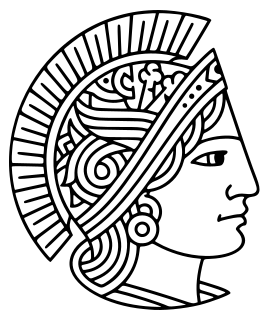
\includegraphics[scale=.12]{images/TUD}%
  %there must be an empty line above this line - otherwise some unwanted space is added between the university and the country (I do not know why;( )
}

\logo{
       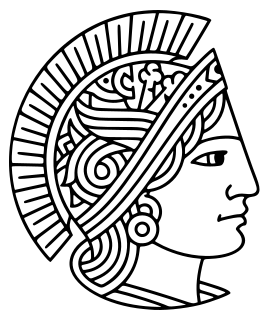
\includegraphics[scale=.03]{images/TUD}%
}

\date{\today}

%\AtBeginSection[]
%{
% \begin{frame}<beamer>
% \frametitle{Inhaltsverzeichnis}
% \tableofcontents[currentsection]
% \end{frame}
%}

%-------------------------------------------------------
% THE BODY OF THE PRESENTATION
%-------------------------------------------------------

\begin{document}

%-------------------------------------------------------
% THE TITLEPAGE
%-------------------------------------------------------

{\1
\begin{frame}[plain,noframenumbering] 
  \titlepage 
\end{frame}}

\begin{frame}{Outline}{}
\tableofcontents
\end{frame}

\AtBeginSection[]
{
	\begin{frame}{Outline}
		\frametitle{Outline}
		\tableofcontents[currentsection]
	\end{frame}
}

%-------------------------------------------------------
\section{Introduction}
%-------------------------------------------------------
\begin{frame}{Introduction}
	\centering
	\begin{figure}[htbp]
		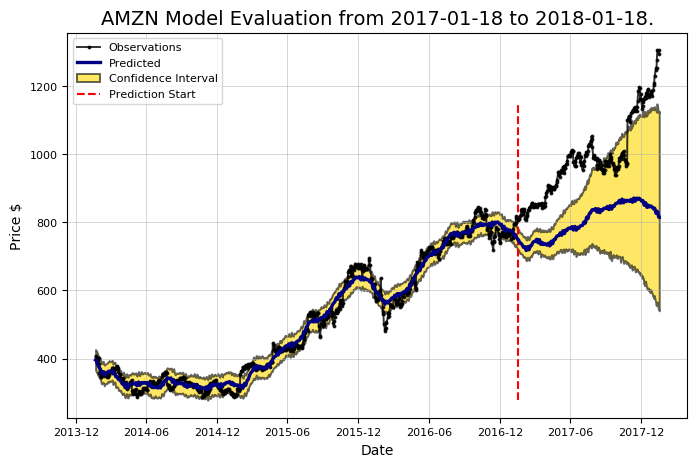
\includegraphics[scale=.35]{images/Motivation}
		\caption{Amazon stock prediction [\textit{https://towardsdatascience.com/stock-prediction-in-python-b66555171a2}]}
	\end{figure}
\end{frame}

%-------------------------------------------------------
\begin{frame}{Introduction}
	\centering
	\begin{minipage}[t]{0.475\textwidth}
		\textbf{Abstract Time Series:}
		\begin{itemize}
			\item What is the overall global trend?
			\item Do I have cyclic patterns?
			\item What are important periods of time?
		\end{itemize}
	\end{minipage}
	\hfill
	\begin{minipage}[t]{0.475\textwidth}
		\textbf{Spatial Time Series:}
		\begin{itemize}
			\item What are regions with unusually high occurrences of events?
			\item How are these regions developing? 
			\item Where are new hotspots occurring? 
		\end{itemize}
	\end{minipage}
\end{frame}

%%-------------------------------------------------------

\section{Abstract Time Series}

%%-------------------------------------------------------

\subsection{An Early Approach}
\begin{frame}{An Early Approach}
	\centering	
	\begin{minipage}[t]{0.475\textwidth}
		\begin{figure}[htbp]
			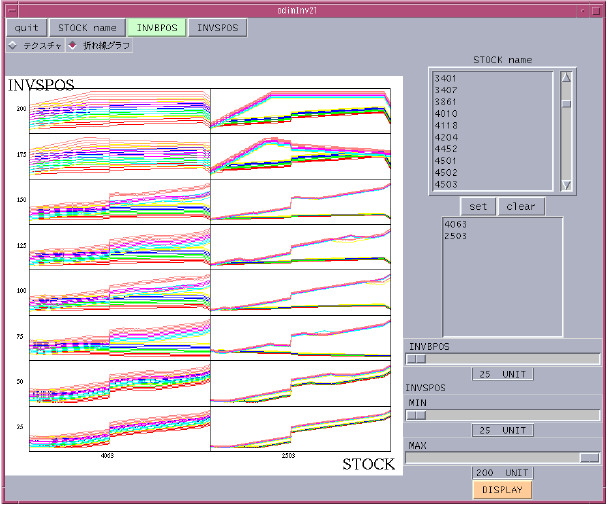
\includegraphics[width=\textwidth]{images/workplace}
			\caption{Workplace environment [\textit{Ichikawa et al., 2002}]}
		\end{figure}
	\end{minipage}
	\hfill
	\begin{minipage}[t]{0.475\textwidth}
		\begin{figure}[htbp]
			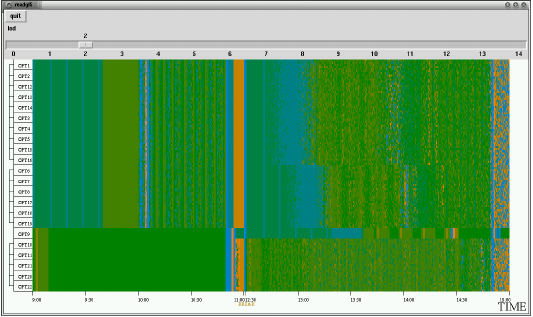
\includegraphics[width=\textwidth]{images/color-band}
			\caption{Color band display [\textit{Ichikawa et al., 2002}]}
		\end{figure}
	\end{minipage}	
	\begin{itemize}
		\item Goal: Trend detection, correlation detection
		\item Compare multiple variables and different time series
		\item External simulations
	\end{itemize}
\end{frame}

%%-------------------------------------------------------
\subsection{A Popular Approach}
%\begin{frame}{A Popular Approach}
%	\centering
%	\begin{figure}[htbp]
%		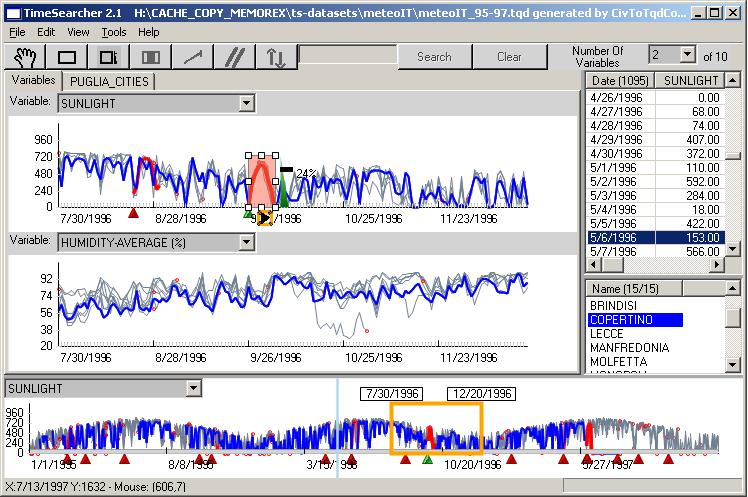
\includegraphics{images/ts2_patternSearch}
%		\caption{TimeSearcher2 pattern search interface [\textit{Buono et al., 2005}]}
%	\end{figure}
%\end{frame}

%%-------------------------------------------------------

\begin{frame}{A Popular Approach}
	\centering
	\begin{figure}[htbp]
		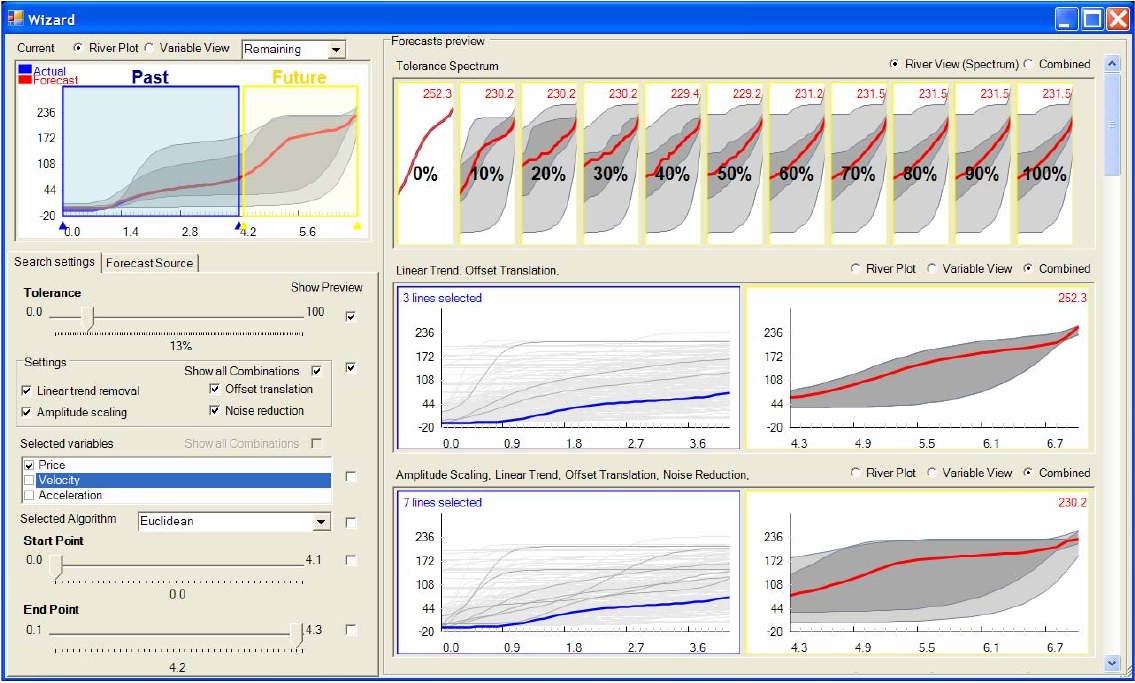
\includegraphics[scale=.17]{images/TimeSearcher}
		\caption{TimeSearcher3 simultaneous preview interface [\textit{Buono et al., 2007}]}
	\end{figure}
	\begin{itemize}
		\item Goal: Model selection
		\item Similarity based model and forecast
		\item Compare different parameters and subsets of data 
	\end{itemize}
\end{frame}

%%-------------------------------------------------------

% TODO Timova
\subsection{A Selective Approach}
\begin{frame}{A Selective Approach}
	\centering
	\begin{figure}[htbp]
		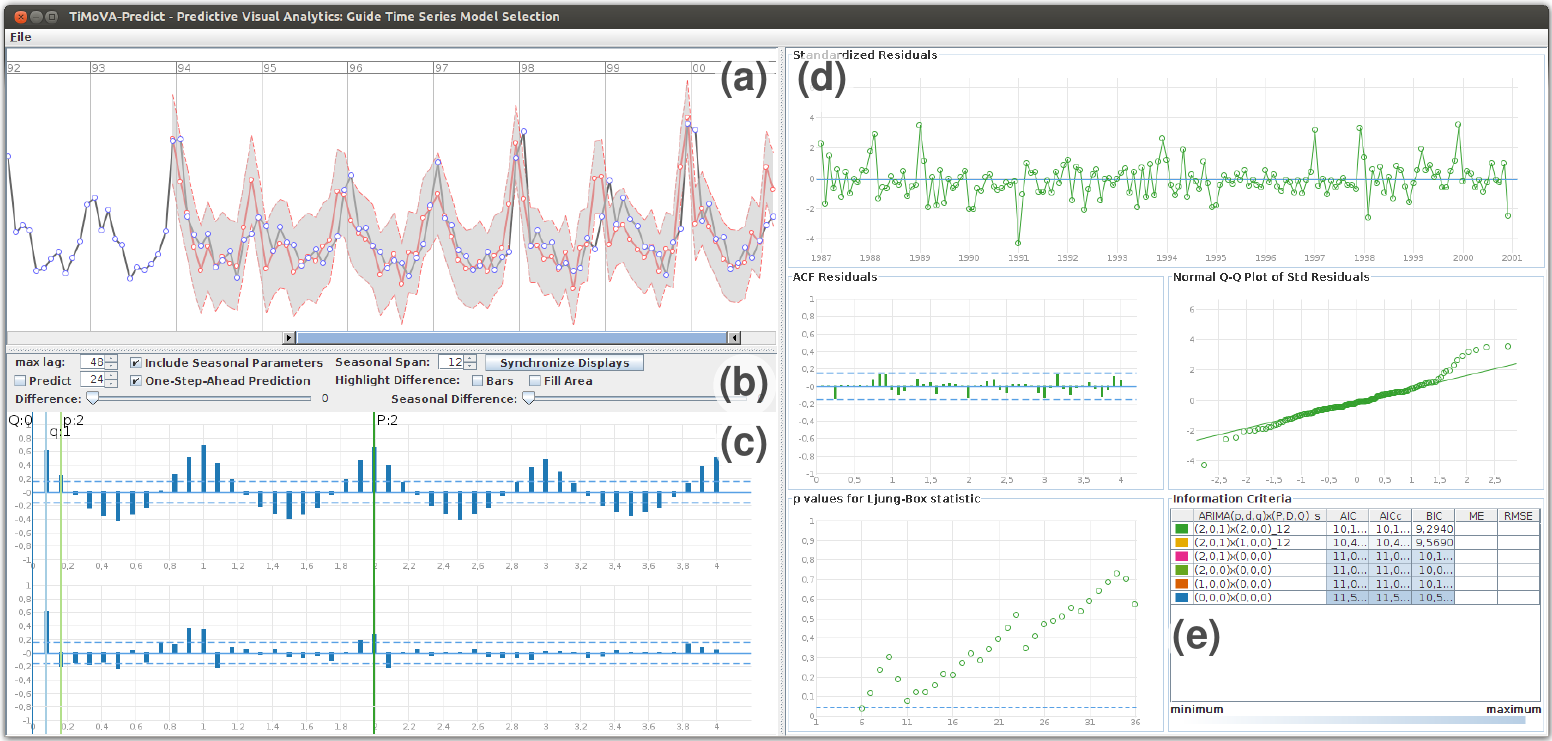
\includegraphics[scale=.17]{images/TiMoVA}
		\caption{TiMoVA User Interface [\textit{B\"ogel et al., 2013}]}
	\end{figure}
	\begin{itemize}
		\item Goal: Model selection
		\item Follows Box-Jenkins-Method
	\end{itemize}
\end{frame}

%%-------------------------------------------------------

\subsection{A Specialized Approach}
\begin{frame}{A Specialized Approach}
	\centering
	\begin{figure}[htbp]
		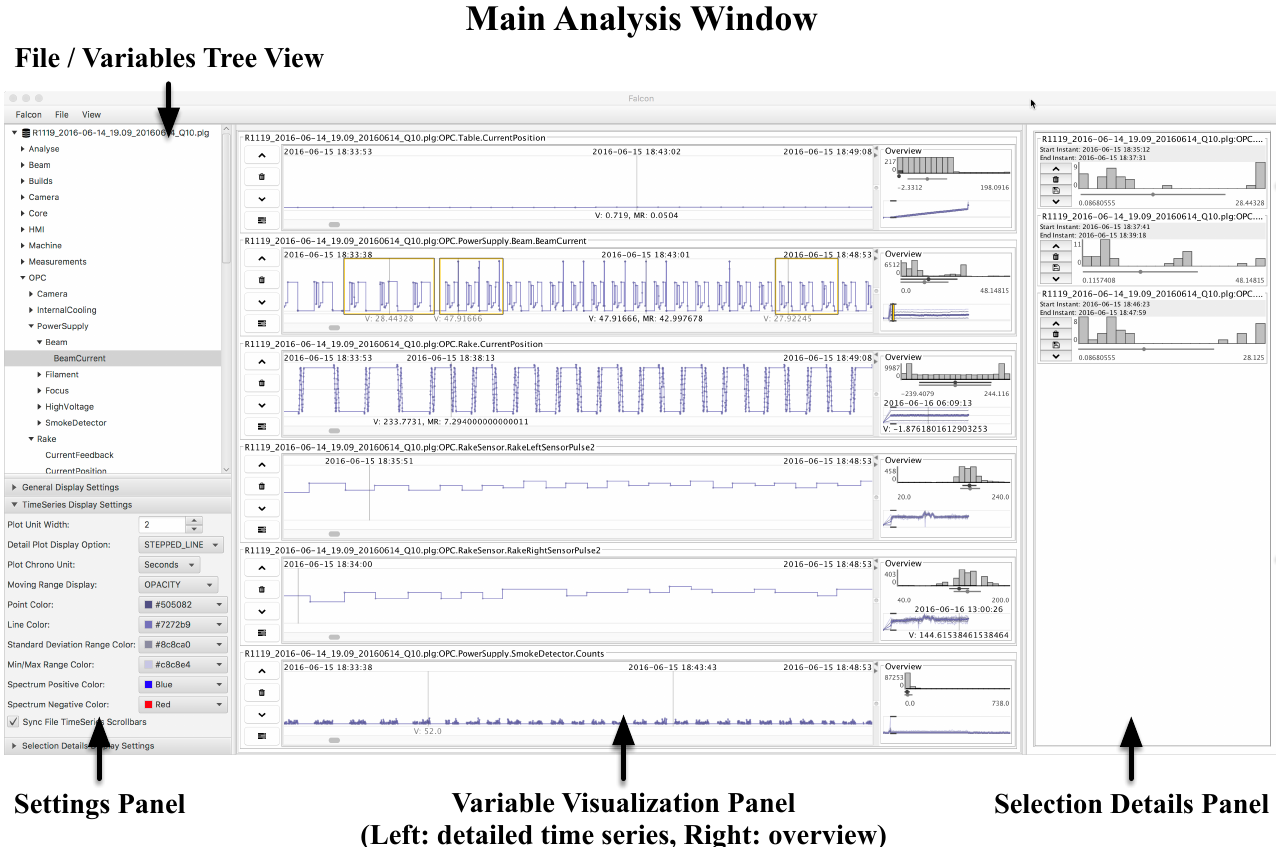
\includegraphics[scale=.2]{images/Falcon_main}
		\caption{Falcon main window visualization [\textit{Steed et al., 2017}]}
	\end{figure}
\end{frame}

%%-------------------------------------------------------

\begin{frame}{A Specialized Approach}
	\centering
	\begin{figure}[htbp]
		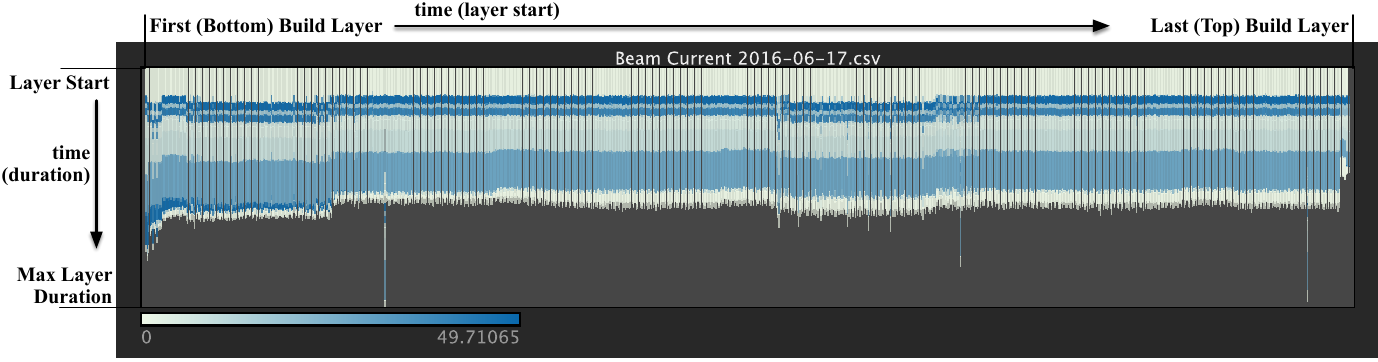
\includegraphics[scale=.22]{images/Falcon_waterfall}
		\caption{Falcon waterfall visualization [\textit{Steed et al., 2017}]}
	\end{figure}
	\begin{itemize}
		\item Find correlations between large amount of variables and time
		\item Application areas: predictive maintenance
	\end{itemize}
\end{frame}

%%-------------------------------------------------------

\begin{frame}{A Specialized Approach}
	\centering
	\begin{figure}[htbp]
		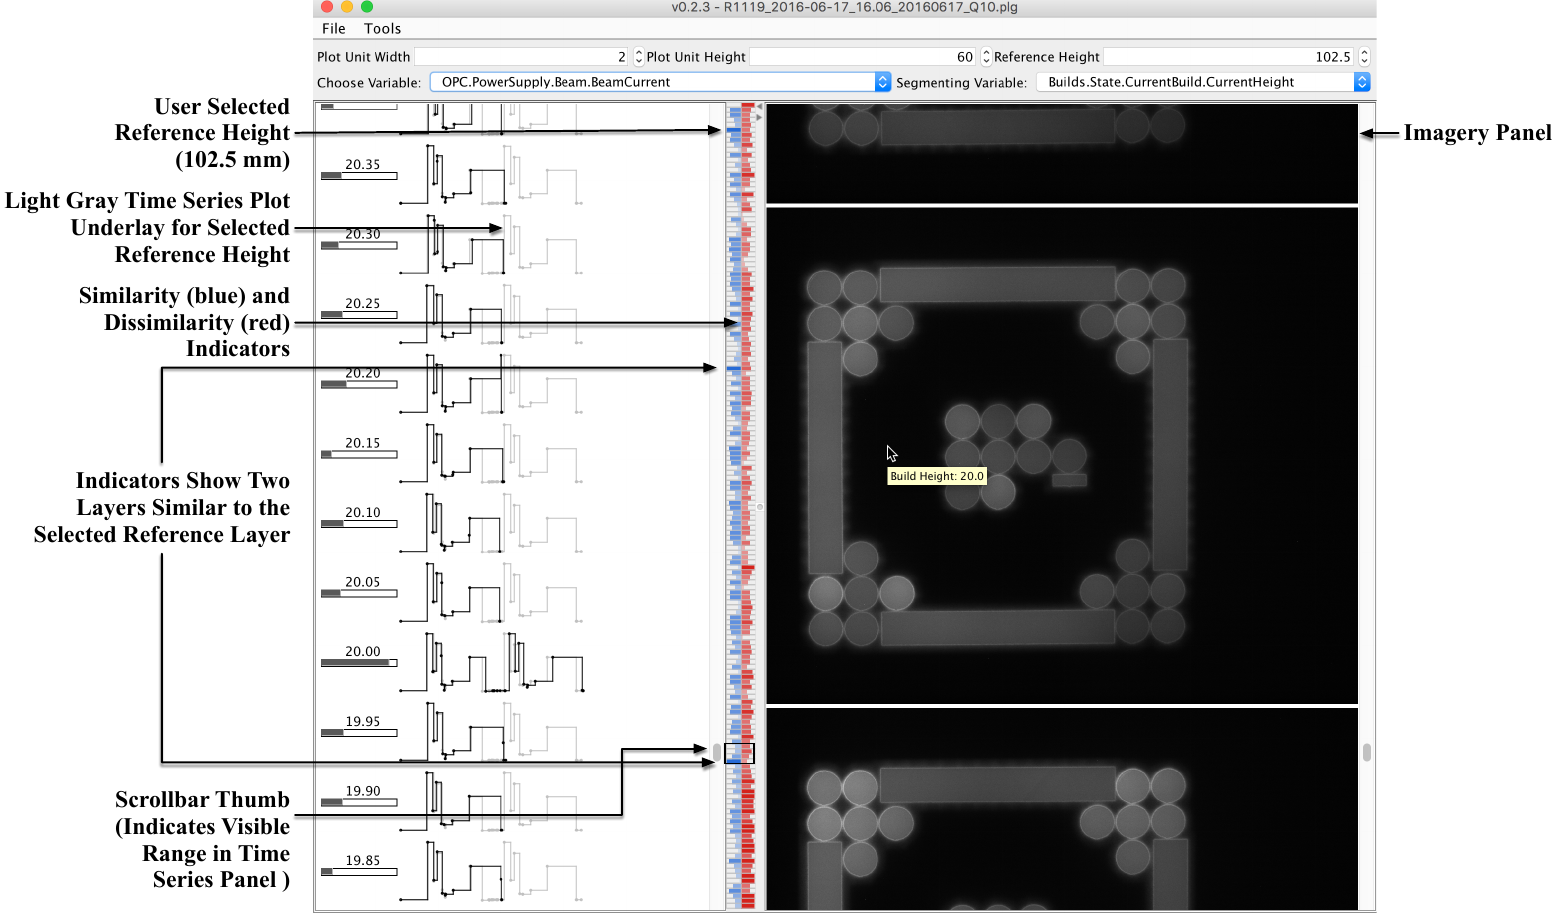
\includegraphics[scale=.18]{images/Falcon_segmented}
		\caption{Falcon segmented time series view [\textit{Steed et al., 2017}]}
	\end{figure}
\end{frame}

\subsection{A Trendy Approach}
\begin{frame}{A Trendy Approach}
	\centering
	\begin{figure}[htbp]
%		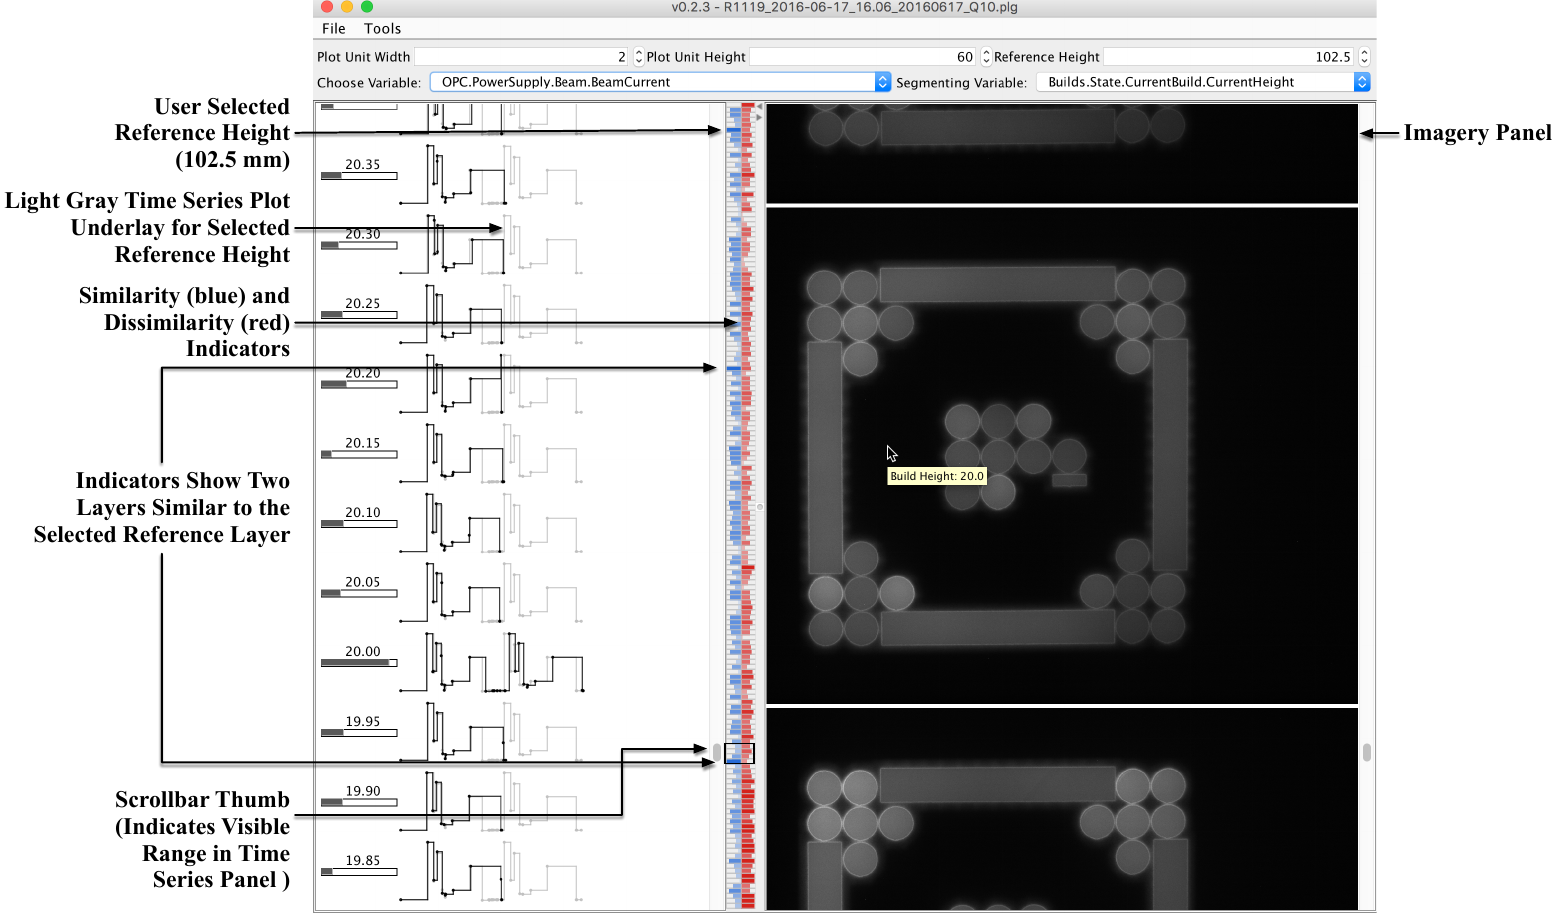
\includegraphics[scale=.18]{images/Falcon_segmented}
%		\caption{Falcon segmented time series view [\textit{Steed et al., 2017}]}
	\end{figure}
\end{frame}

%%-------------------------------------------------------

\section{Spatial Time Series}
\subsection{Forecasting and Detecting Hotspots}
\begin{frame}{Forecasting and Detecting Hotspots}
	\centering
	\begin{minipage}[c]{0.65\textwidth}
		\begin{figure}[htb]
%			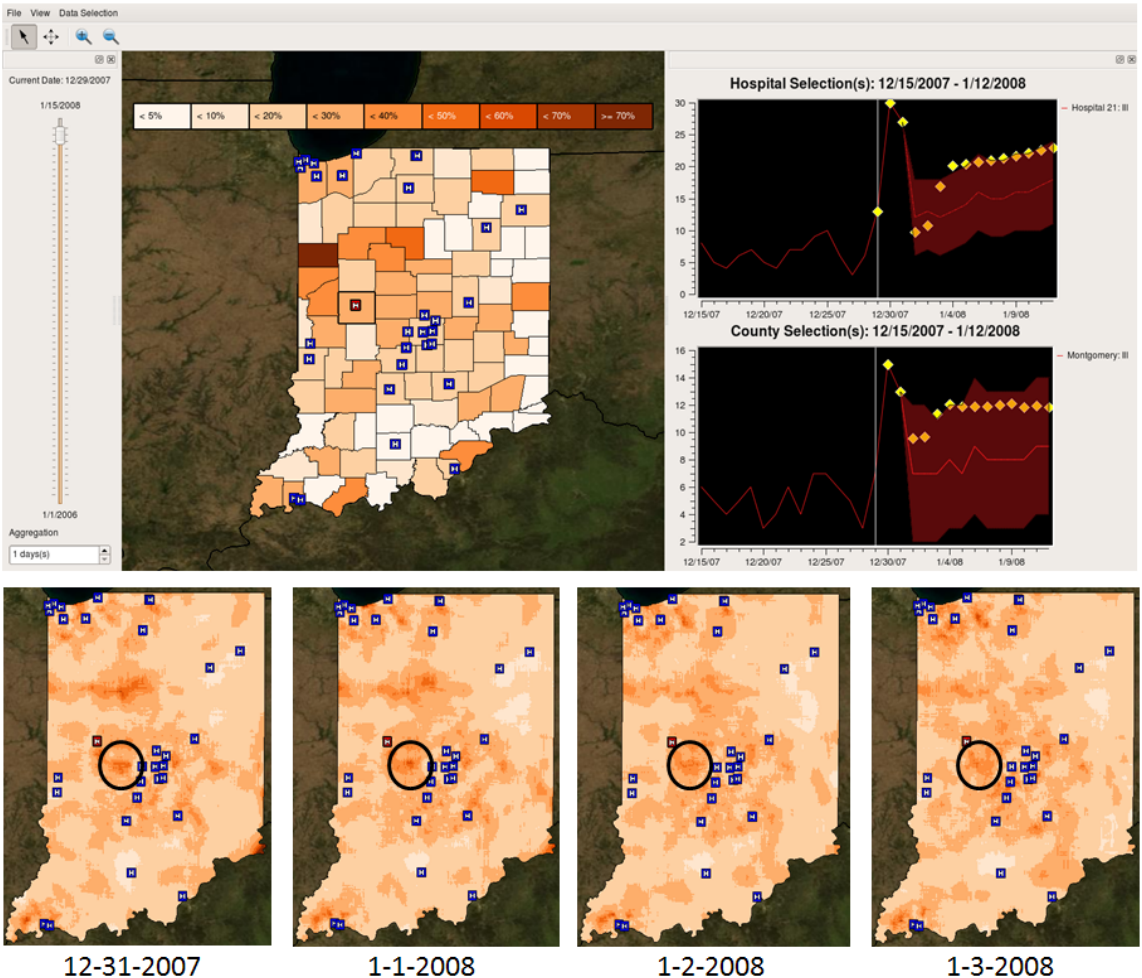
\includegraphics[scale=.16]{images/Hotspots_larger}
			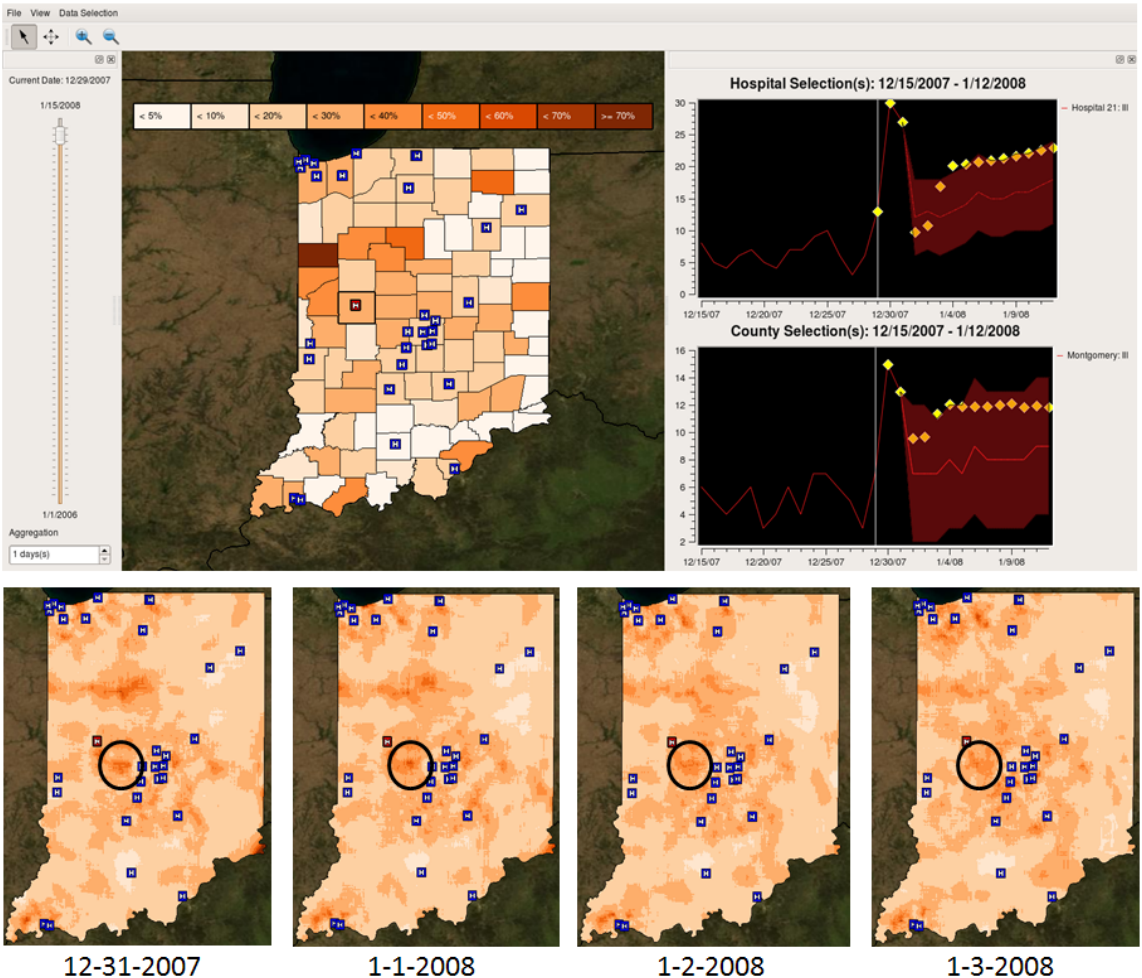
\includegraphics[width=\textwidth]{images/Hotspots_larger}
			\caption{Forecasting Hotspots [Maciejewski et al., 2011]}
		\end{figure}
	\end{minipage}
%	\hfill
	\begin{minipage}[c]{0.325\textwidth}
			\begin{itemize}
				\item Model based spatial approximation
				\item Direct linkage of time series prediction with spatial information
				\item Main focus: Hotspot detection and prediction
			\end{itemize}
	\end{minipage}
\end{frame}

%-------------------------------------------------------
\subsection{Mapping between Time and Space}
%\begin{frame}{Separation of Temporal and Spatial}
%	\centering
%	\begin{figure}[htbp]
%		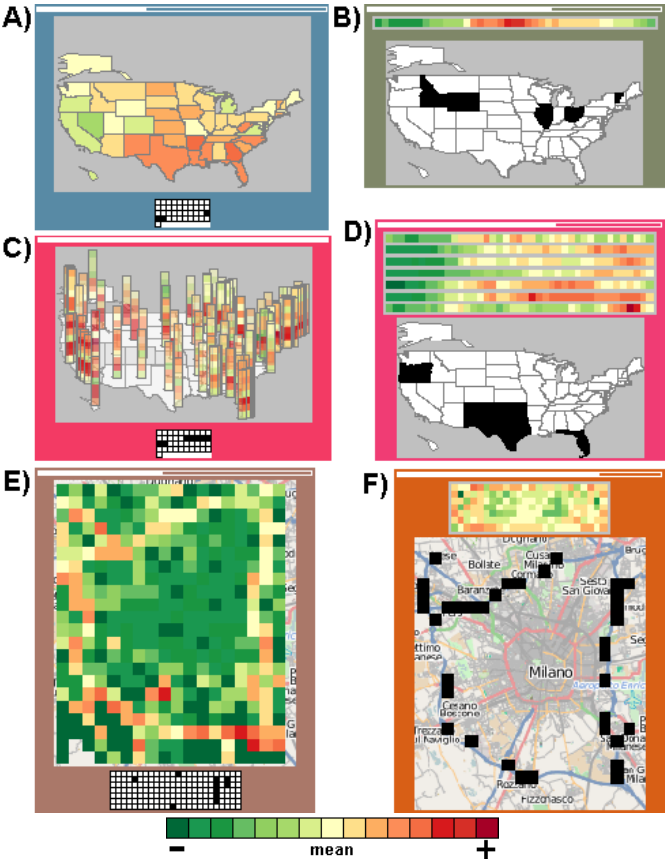
\includegraphics[scale=.2]{images/SOM}
%		\caption{Possible cell appearances [\textit{Andrienko et al., 2010}]}
%	\end{figure}
%\end{frame}

%-------------------------------------------------------

\begin{frame}{Mapping between Time and Space}
	\centering
	\begin{minipage}[t]{0.475\textwidth}
		\begin{figure}[htbp]
			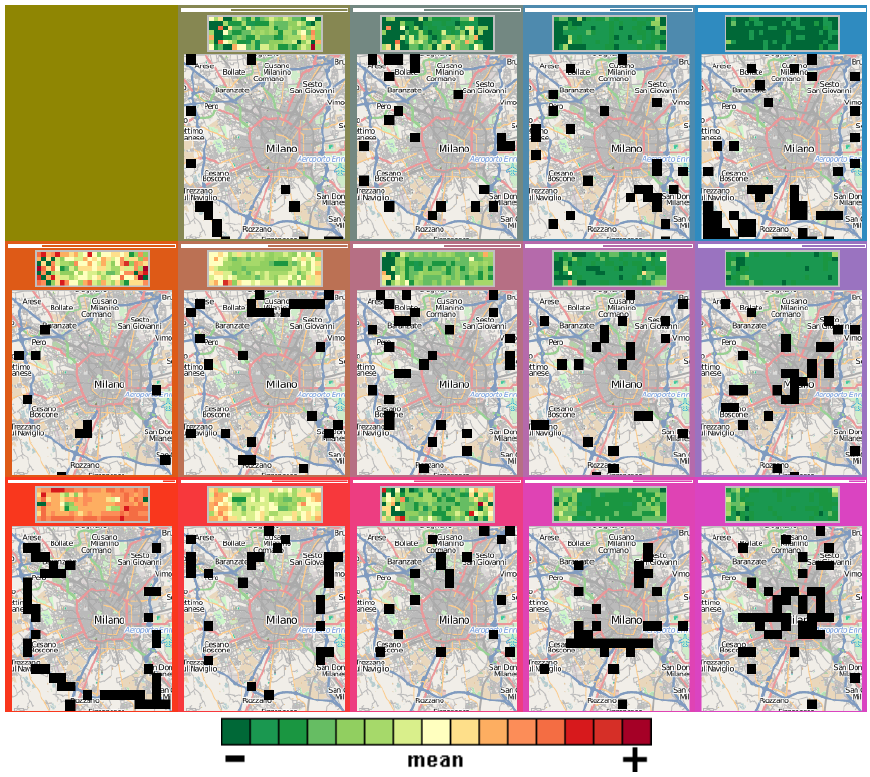
\includegraphics[width=\textwidth]{images/SOM_SiT}
			\caption{Time-in-space matrix [\textit{Andrienko et al., 2010}]}
		\end{figure}
	\end{minipage}
	\hfill
	\begin{minipage}[t]{0.475\textwidth}
		\begin{figure}[htbp]
			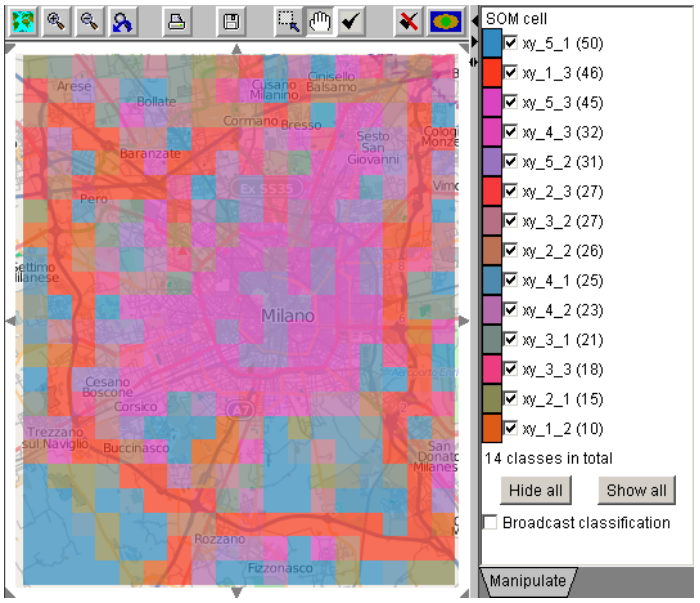
\includegraphics[width=\textwidth]{images/SOM_map}
			\caption{Spatial mapping of Time-in-space matrix [\textit{Andrienko et al., 2010}]}
		\end{figure}
	\end{minipage}
	\begin{itemize}
		\item Clustering on spatial or temporal level
		\item Direct linkage of time series prediction with spatial information
	\end{itemize}
\end{frame}

%-------------------------------------------------------

\begin{frame}{Summary}
	\begin{itemize}
		\item Turning points, seasonality and outliers make predictions complex
		\item How to deal with really large amounts of data?
		\item How to preserve peaks?

%		\item Visualizing high dimensional time series is hard
%		\item Visual Analytics helps to understand the data
%		\item Finding patterns is important for prediction
%		\item Predictive systems are often limited to specific application areas
%		\item Analyzing Spatiotemporal data is complex and requires human analysts as well as software tools
	\end{itemize}
\end{frame}

%-------------------------------------------------------

\begin{frame}[allowframebreaks]{Bibliography}
		\nocite{buono:2007}
		\nocite{steed:2017}
		\nocite{ichikawa:2002}
%		\nocite{Lu:2017}
		\nocite{boegl:2013}
		\nocite{boegl:2014}
		\nocite{maciejewski:2011}
		\nocite{Andrienko:2010:Space}
		\bibliographystyle{plain}
		\bibliography{bibliography}
\end{frame}

%-------------------------------------------------------

{\1
\begin{frame}[plain,noframenumbering]
  \finalpage{Thank you for listening}
\end{frame}}

\end{document}